\documentclass{vldb}
\usepackage{graphicx}
\PassOptionsToPackage{hyphens}{url}\usepackage{hyperref}
\usepackage{gensymb}
\usepackage{balance}  % for  \balance command ON LAST PAGE  (only there!)
\usepackage[multiple]{footmisc} %multiple footnotes
\usepackage{chngcntr}
\counterwithin{table}{section}
\counterwithin{figure}{section}


\begin{document}

% ****************** TITLE ****************************************

\title{Travel Buddy: Exploring the world with remotely controlled drones}

\numberofauthors{2}

\author {
\alignauthor
Ondrej Borovec\\
       \affaddr{Czech Technical University in Prague}\\
       \affaddr{Prague, The Czech Republic}\\
       \email{o.borovec@gmail.com}
\alignauthor
Jan Zaloudek\\
       \affaddr{University of Massachusetts in Lowell}\\
       \affaddr{Lowell, MA}\\
       \email{Jan\_Zaloudek@student.uml.edu}
}

\date{30 April 2017}

\maketitle
\begin{abstract}
Tourism and and travel industry makes still growing field which contributes a lot of money to Global GDP. Even thought exploring of the world has never been easier there are still many people for who it is too complicated to use this opportunity. We are proposing a solution based on combination of remotely controlled drone and VR which maximizes impression of travelling to people with limited mobility or with any kind of problem which stops them from sharing a special remote moment of their relatives and friend. We are also focused on evaluation of user satisfaction  for further  service development.
\end{abstract}




\section{Problem Statement}
Travel and tourism industry contributed around 7.61 trillion USD to world global economy in 2016\footnote{https://www.statista.com/topics/962/global-tourism/}\footnote{http://www.hospitalitynet.org/news/4069673.html} and it is steadily growing field with big potential. According to a BBC article published in 2013\footnote{http://www.bbc.co.uk/schools/gcsebitesize/geography\newline/tourism/tourism\_trends\_rev2.shtml} the main reasons of tourism growth are: more affluence, greater awareness, more leisure time and more choice. These features are mostly mentioned in connection to more industrialized and wealthy continents as Europe or North America, but it last year, other continents and counties are decreasing the difference which opens the tourism market even more.

As we can see in the figure \ref{fig:touristsPerYear} there are many people who are travelling because of tourism, but compare to the total number of people on the Earth there are more who cannot travel and it can be due to several reasons. The biggest one would definitely be lack of money, for instance, in 2013 still 14.5\% of all Americans, lived below the poverty line. We do not think that a single technology improvement can solve this problem and it is also not the point of this paper. We would like to focus on people who cannot travel because lack of time, mobility problems or age.

According to Darcy and Dickson\cite{darcy2009whole} up to 30\% of a population will have higher access requirements at any point in time during their lives which can affect their ability to travel. This percentage does not cover only missing limbs, but also requirements of some elder to visit their doctors frequently of dependency on medicament. We believe, people with some limitations deserve to get back the feeling of equality and gain back their dignity. We feel it is important to open the gates of the world to as many people as possible, so people can open their eyes and start care about out blue plane even more. 

There is also another aspect which significantly influences current world tourism - Security and terrorism - as was studied at \cite{bac2015terrorism}. According to this study tourism industry has not fully recover after the incident in 2001 and with the reason that people did not gain their full trust to security system. But, unfortunately, there is no study, how many people would travel more if it would be a danger-free

The most real-experience solution for remote virtual tourism would be a humanoid robot controlled by Virtuix Ommi system\footnote{http://www.virtuix.com/product/omni-package/}. Unfortunately, required robot technology does not exist and even if it would, price of needed technology cause that it would be only for the rich people. Another fact is that, this would not make traveling easier for the people, we would like to focus on. Virtuix system relies on full movement of your body and cannot be controlled by people who have mobility problems and have a problem with real travelling.

We are experiencing rapid technology development of drone and virtual reality technology. In the last years, several companies introduced how innovations can be used in industry and services. For instance, Amazon was to use drones for delivering\footnote{http://money.cnn.com/2017/02/14/technology/amazon-drone-patent/} and VR is used for surgery practising\cite{nagendran2013virtual} or pilot training\cite{grabowski2015virtual}, but the main usage of drones and virtual reality is in entertainment. We would like to suggest less costly solution for visiting of remote places via remotely controlled drone with VR system.

Problematic of VR and drone technology has been solved on its own, but combining these technologies bring a lot of difficulties. Current industry drones are controlled by a joystick controller, which according to \cite{mangina2016drones} may allow you maximum control, but learning curve is not sufficient for not frequent users.The paper suggests controlling headset, which is more intuitive (figure \ref{fig:OculusRiftSensorSetup}) and can also be enriched by VR extension. 

Another problem which is also studied at \cite{mangina2016drones} is controlling of remote object which distance from the person who is driving it is changing. It may cause changes in response time of controlled device, in our case drone, and this latency problem can also appear with controlling over an internet connection. This overall problem is also well described and studied at \cite{benjamin2013drone}.

The goal of this paper is to suggest a technical solution which would allow people with any mobility or mental problems to share traveling experience of their relatives and friend. We would like to show, how it is possible to provide at least similar experience of traveling thanks to modern technology with maximum interaction with real surrounding world and freedom to move. Another important aspect is that such solution should not be expensive, so it is affordable for maximum community.

\begin{figure}[t]
    \centering
    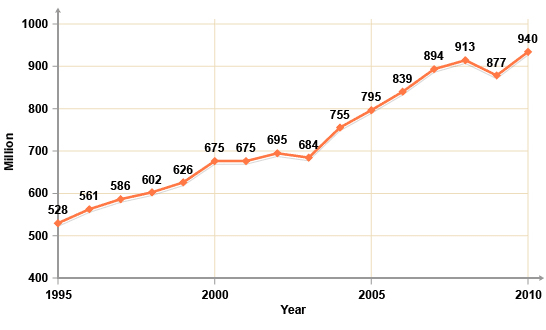
\includegraphics[width=0.40\textwidth]{img/worldTouristsPerYear}
    \caption[Number of tourists per year between 1995 and 2010]{Number of tourists per year between 1995 and 2010\footnotemark}
    \label{fig:touristsPerYear}
\end{figure}
\footnotetext{\url{http://www.bbc.co.uk/schools/gcsebitesize/geography/tourism/tourism\_trends\_rev1.shtml}}

\begin{figure}[t]
    \centering
    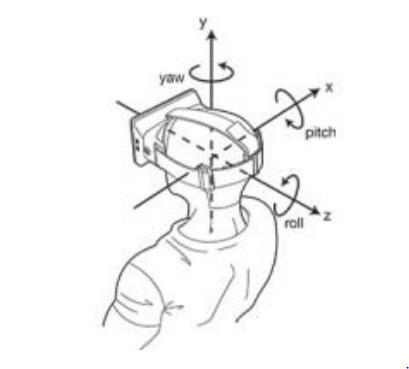
\includegraphics[width=0.40\textwidth]{img/OculusRiftSensorSetup}
    \caption[Oculus Rift Sensor Setup]{Oculus Rift Sensor Setup}
    \label{fig:OculusRiftSensorSetup}
\end{figure}







\section{Related Work}
Virtual reality as we know it today is around since 1990's, when in 1991 Sega released its first VR headset \cite{sega2004headset}. Since then a lot of research has been done however VR headsets were sidelined. In 2012 Oculus presented modern headset for consumers and thanks to the greater computing power of today's computers and smartphones, the idea of virtual reality became popular again.

In 2013 DJI released their first consumer-grade drone with integrated camera. Until then drones were large, expensive and available to mainly to professionals. Since then many companies have become more focused on drones and they have developed rapidly since then.

In further sections we will discuss and compare different existing solutions that include drones, virtual reality or virtual travelling.

\bgroup
\def\arraystretch{1.5}
\begin{table*}[t]
\centering
\begin{tabular}[c]{r|p{2cm}lllp{3cm}}
                         & DJI                         & YouVisit   & Facebook VR & Viooa                        & Limited mobility          \\ \hline
Data transfer technology & WiFi and Lightbridge        & Internet   & N/A         & N/A                          & Wifi (802.11n)            \\
Range                    & up to 7km                   & $\infty$   & N/A         & N/A                          & $\sim$50m                 \\
Latency                  & 110ms                       & Depends    & N/A         & N/A                          & $\sim$Good enough         \\
Camera                   & wideangle camera on gimball & 360\degree & N/A         & 360\degree$\times$180\degree & N/A                       \\
VR headset               & DJI Goggles                 & Any        & Oculus Rift & No                           & Oculus Rift               \\
Controlling camera       & Yes, head movement          & Partialy   & N/A         & Software based               & No                        \\
Controlling drone        & Remote controller           & N/A        & N/A         & N/A                          & Yes, 6 DOF, head movement
\end{tabular}
\caption{Comparison of available solutions}
\label{solutions-comparison}
\end{table*}
\egroup

\subsection{YouVisit}
Website called YouVisit\footnote{\url{https://www.youvisit.com}} is a virtual travelling service. They provide virtual tours to the different parts of the world through 360\degree video footage. Users can look around in the scene by using their mouse in the web browser or they can use any compatible VR headset.

\subsection{Google Streetview}
Google Maps\footnote{\url{https://maps.google.com}} provide a feature for exploring different locations through 360\degree camera which is mounted on the roof of the car. Users are able to move on the map and look around. They have implementation for web browser, controlled by mouse and also a version for phone-based VR headsets.

\subsection{DJI Goggles}
DJI is currently the leader in consumer and professional drones production. Their product called DJI Goggles\footnote{\url{https://www.dji.com/dji-goggles}} is actually wireless remote screen for the drone's camera. The camera is mounted on a small gimbal on the bottom of the drone and its movement is controlled by the sensors placed in the goggles. Drone itself is controlled by another person with the remote controller or it can fly in one of the many fully automatic modes. The advantage of this solution is relatively small latency ($\sim$110ms), thanks to their technology Lightbridge. On the other hand the signal range is quite limited (units of kilometers), therefore it cannot be fully used for travelling purposes.

\subsection{Facebook VR}
Since Facebook bough Oculus in 2014 it has become one of the major companies responsible for the recent research in the field of VR. They do not provide any complex solution for our proposed problem, but they have a variety of devices and technologies that can be used.

At first Facebook provides solution for transferring 360\degree video by decreasing an amount of transferred data by increasing compression of the image out of the user's viewport \cite{facebook2016videoencoding}. This solution is based on mapping an image onto pyramids and reduces transferred data for about 80\%. 

Secondly, they produce state-of-the-art VR headset Oculus Rift, which can be easily connected to the computer and be used as a display for the drone footage. Thanks to the integrated sensors (accelerometer, magnetometer and gyroscope) it can provide the necessary data for controlling the drone.

\subsection{Viooa}
Viooa is 360\degree camera\footnote{\url{http://www.viooa.com/}}, primarily to be used for drones. It reduces the necessity of a gimbal, which is used for current drones to stabilize the image and pan around with the camera. Their implementation is capable of advanced 3D mapping and stabilizing the footage without using any moving parts.

\subsection{Streaming for people with limited mobility}
Team behind this paper proposed solution for people with limited mobility. They used Oculus Rift headset and Wii Nunchucks to monitor head movements and used values from those sensors to navigate the drone \cite{mangina2016drones}. They run a couple of experiments with different setups and end up with a solution based on the Oculus Rift. The downside of this implementation is the range of the drone. Their drone uses just the WiFi and to maintain latency low enough to operate drone comfortably, the range of the drone is approximately 50 meters from the signal source\cite{mangina2016drones}.

\subsection{Comparison}
The best solution so far for the drone with the VR headset is probably DJI Goggles, which provides a lot of functionality for controlling camera and the drone. On the other hand the best solution for actual travelling is YouVisit, where users can see what is happening thousands kilometers away from them. Other solutions solve just smaller parts of the more complex problem. Features of current solutions are shown and compared in table \ref{solutions-comparison}




\section{Proposed Solution}
Building such a platform from scratch can be quite expensive while there are many parts that can be integrated together. Integration of different parts together can reduce the price significantly. There are two main parts of our solution. There is a drone and its controller on one side and the VR headset with sensors on the other side. They are connected together through the Internet, so the latency greatly depends on the quality of your connection. That is why we decided to use 360\degree camera instead of a traditional drone camera placed on gimbal. We can transfer 360\degree video with large compression of areas, which are out of viewers viewport. This can be done by mapping image onto the pyramids and therefore reduce the amount of transferred data by 80\%\cite{facebook2016videoencoding}.

\subsection{Drone and controller}
For building a prototype it is easier to start with some kind of a drone kit. Therefore, we chose quadrocopter with mounts for the other hardware and camera\footnote{\url{http://www.robotshop.com/en/lynxmotion-hquad500-drone-base-combo-kit-quadrino-nano-controller.html}}. It is definitely more expensive than having a drone with all hardware integrated in one body, but for the purpose of future tweaking of our idea, the kit is better. 

Chosen controller contains GPS, accelerometer, gyroscope and accelerometer and it would be possible to pair this controller with autopilot module\footnote{\url{http://www.robotshop.com/en/navio2-autopilot-kit-raspberry-pi-2-3.html}}. Autopilot module is optional, but for our experiments it would be necessary. During the experiments we want to find out, which way of controlling drone is easier for the users. If there is big latency in communication, the autopilot can be the way to go. It can be also connected together with Viooa camera and drone, then can provide features such as tripod mode, follow me mode or fly around.

For the success of this solution is crucial battery life. Therefore, we have to integrate battery that allows drone at least 20 minutes of flight. This item can be adjusted as we need, but from the start, we chose battery with 3500 mAh\footnote{\url{http://www.robotshop.com/en/111v-3500mah-30c-lipo-battery.html}}.

\subsection{Camera}
For our solution we decided to use 360\degree$\times$180\degree camera Viooa\footnote{\url{http://www.viooa.com/viooa.html}}. This camera shoots 4k footage and integrates a lot of smart algorithms that can help with controlling the actual drone.

This camera can be mounted to the bottom or the front of the drone and the image from the camera will be streamed over the WiFi to the phone and then over the Internet right to the VR headset.

\subsection{VR headset}
We chose Oculus Rift VR headset\footnote{\url{https://www.oculus.com/rift/}}, which supports all features we need and furthermore it also has touch controls Oculus Touch. Touch controls can be used for fine drone controlling or it can be used by people, who have limited head movements. 

\subsection{Software}
To transfer data between the drone and a viewer we have to implement software, which will be able to operate with high amount of data. To compress the data, we want to use Facebook's implementation of 360\degree video, that maps the original footage to the multiple pyramids and saves a huge amount of data\cite{facebook2016videoencoding}. We also have to implement a system, that deals with the latency of the connection and it can be quite challenging. Other solutions, such as DJI Goggles, are dealing with few kilometers of distance (at maximum) and they keep latency at 100ms only when the drone is on sight.

The actual implementation of client and server software will be done upon a larger discussion. Current proposed solution can serve as a framework for further work.

\subsection{Other requirements}
The most crucial requirement for pleasant experience is good internet connection between the drone and the viewer. Thanks to the modern mobile technologies, we are now able to transfer large amount of data over the mobile networks with a decent latency. Our architecture proposal can be seen on figure \ref{fig:connection}.

\begin{figure}[h!]
    \centering
    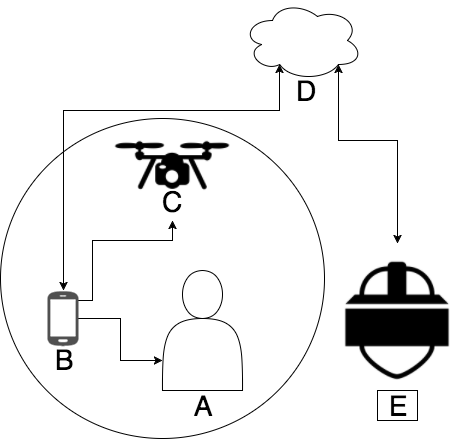
\includegraphics[width=0.40\textwidth]{img/connectiondiagram}
    \caption[]{Diagram of system architecture:\newline A - Traveller, B - Mobile device, C - Drone,\newline D - Clouse service, E - Pilot with controlling headset}
    \label{fig:connection}
\end{figure}

\subsection{Price}
Price is probably something, what can be reduced with further development of the product and integrate all the components in the one body. Price can be split between drone and VR headset, because many people can already have some kind of compatible headset they can use. Detailed prices of the components are shown in table \ref{estimatedprice}.

\bgroup
\def\arraystretch{1.5}
\begin{table}[h!]
\centering
\begin{tabular}{p{4}p{2.5cm}}
\textbf{Item}                                                          & \textbf{Estimated price (USD)} \\ \hline
\multicolumn{2}{l}{\textit{Drone}}                                                             \\ \hline
\multicolumn{1}{l|}{Drone body + controller}                  & 520 (+250 for autopilot)                   \\
\multicolumn{1}{l|}{Viooa 360\degree camera (or alternative)} & $\sim$700             \\
\multicolumn{1}{l|}{Remote control}                           & 130                   \\
\multicolumn{1}{l|}{Battery \& other drone modules}       & 100                   \\ \hline\hline
\multicolumn{2}{l}{\textit{Viewer}}                                                            \\ \hline
\multicolumn{1}{l|}{Oculus Rift}                              & 600                   \\ \hline\hline
\textbf{Total}                                                         & \textbf{2300}                  \\ \hline
\end{tabular}
\caption{Estimated price of prototype}
\label{estimatedprice}
\end{table}
\egroup


\section{Evaluation Methodology}
In this paper, we described a possible solution of sharing realistic travel experience for people with any kind of mobility problem. In this section we describe the methodology, how to evaluate whether out control setting is user friendly and then we want to estimate overall user satisfaction.

\vspace{40pt}
\subsection{Control device preferences}
Comparison of controlling headset and a classic joystick device has been done in \cite{mangina2016drones} with the results that a headset is more intuitive and has a better learning curve for amateur drone pilots. But their testing does not fully follow our proposed concept, because there were using there two ways of controlling with direct eye contact with the controlled drone. For our purposes, we need to update the test condition so that pilots can see only what is displayed to the VR device.

Each participated in the test group will have to pilot two flights: one with the classic hardware controller and one with the headset controller, but with the same trajectory description. The instructions are to take off, follow a predefined trajectory around a moving object and land on a predefined spot. We considered several approaches how to evaluate the effectiveness of the controlling systems. We see total time of a flight and precision (stability, fluency, ...) as the most important features, but we also want to visually evaluate emotional reactions during of tested subjects and surveys which are made afterwards. We also can use a cam and image processing to identify marks of frustration or stress.

This test should be taken several times to identify learning curve of both controlling devices. Or we can add a condition, that pilot has to participate in a conversation so we can evaluate, how good are pilot using one of other control way with side human interaction. This aspect is also very important, since we want to provide maximum human friendly travel experience.

\subsection{User satisfaction}
The second evaluation focuses on user overall satisfaction with our solution. It is really hard mission to estimate comparable metric for this experiment since everybody has perception. We agreed there is no was a controlled laboratory experiment could have a proving value, so the best way is to analyze usage of several free-give-away prototypes. People for this test have to be selected wisely, such people has to travel a lot and also has to have some relatives who would like to travel with and but cannot. It means a background check i needed. The advantage of this real world experiment is that it can even continue after the prototype testing, we could monitor our user with their awareness to continuously improving our services.

Possibly monitored features (using term traveller for a person who has receiving mobile device and term pilot for person who remotely control the connected drone using our proposed headset):
\begin{itemize}
  \item General statistical observation like usage per time period, average time of usage, number of different users of a prototype, ...
  \item After every session there will be an optional survey in which pilots and travellers can express their feeling about their last session. The survey may contain questions related to session itself like connection quality, control delaying, ...; to the place where pilot was present (session took place) like how propriety is that place, how hard is to navigate there, ...; and to users mood and expectations. To make it easier and faster, questions should be able to answer using a predefined scale.
  \item Since our solution includes voice transmission between a traveller and pilot, we can analyze tones of their voices to determine mood of their conversation. 
  \item One of the main advantages of our solution is direct interaction between a traveller and a pilot, it means that the camera which is placed on the drone will sometimes capture traveller's face. Then we can use image processing to determine traveller excitement of sharing that moment. 
\end{itemize}

Collecting this information we can create a big dataset. It is unlabeled data in the beginning, so we would need to label some of them by hands. After that we can use modern machine learning methods to label newly collected data.

\bibliographystyle{abbrv}
\bibliography{biblio}  


\end{document}
